\frame{
  \frametitle{Red Black Tree\footnote{Guibas, Leonidas J.; Sedgewick, Robert (1978).}}
  \begin{columns}
      \begin{column}{0.5\textwidth}
          \begin{itemize}
            \item Balanced BST, red-black coloring chosen because it looked best on the laser printer they used.
            
            \medskip
            
            \item All root-to-leaf paths have the same number of black nodes

            \medskip
            
            \item No red node has a red parent
          \end{itemize}
      \end{column}
        \begin{column}{0.5\textwidth}
            \begin{center}
                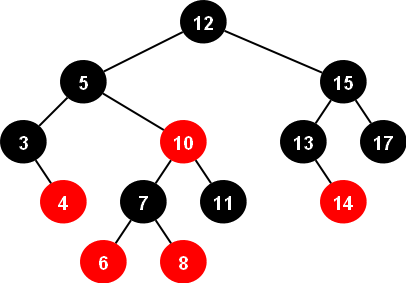
\includegraphics[scale=0.3]{slides/alphabet_trees/redblacktree.png}

                {\tiny \texttt{https://pages.cs.wisc.edu/\texttildecenter wyoungjun/}}
            \end{center}
        \end{column}
  \end{columns}
    
}